\title{Lab 2: Temperature Sensing}
\author{Engineering 100-950}
\date{Winter 2020}
\documentclass[12pt]{article}
\usepackage[margin=1in]{geometry}
\usepackage{fancyhdr}
\usepackage{siunits}
\usepackage{hyperref}
\usepackage{circuitikz}
\chead{Written and Edited by Arun Nagpal, Aaron Ridley, Scott Smith, Lyndon Shi, Kitty Ascrizzi, and Sarah Redman}
\usepackage{graphicx}

\begin{document}
	\maketitle
	\thispagestyle{fancy}
	
	\section*{Materials}
	\begin{itemize}
		\item 1 \quad Arduino Nano
		\item 1 \quad TMP36 Temperature Sensor
		\item 1 \quad B57164K Amtherm Thermistor
        \item 1 \quad 1 k$\Omega$ Resistor
		\item 1 \quad Sparkfun OpenLog
		\item 1 \quad Sparkfun Level-Shifter
		\item 1 \quad SD Card
	\end{itemize}
	
	\section*{YouTube Video}
	\href{https://www.youtube.com/playlist?list=PLp2z0IQxLSvkzzYafHIlGQl9MbUdtYAeH}{We highly recommend that you watch the following YouTube video playlist (click here) prior to lab. Part 1 helps explain ADCs. We talk about the temperature sensor in part 2 at time-stamp 4:55.}\\
	
	\href{https://www.youtube.com/watch?v=FhgAi-ju6Z4}{Additionally, this video (click here) should help you better understand the OpenLog and Level-Shifter used in this lab.}

\section*{Introduction}
	This lab represents the start of your journey into the development of your high altitude sensor board. Your board will measure an ensemble of atmospheric variables, including temperature, pressure, humidity, acceleration vector, and location information. We will begin with the simplest, most visceral metric: temperature. This lab will introduce you to the temperature sensor associated with your sensor board.\\
	
	A \textbf{sensor} is a device that provides measurement of some environmental observable. Many times, sensors work by \textbf{transduction} whereby they convert one form of energy into another, often times converting input to electrical energy. However, how do we know what the relationship is between the input and the output? If, for instance, the output from a temperature sensor reads as 2 Volts at room temperature, what does an output of 3 Volts mean? In order to answer this question, we need to generate a \textbf{calibration curve} for the sensor: an equation that maps input values against output values.\\
	
	Here's a cool example: since you'll be dealing with a temperature sensor this lab, check out these calibration curves for different flavors of a temperature sensor that relies on a physical process called the thermoelectric effect. When two dissimilar metals are brought into contact, a voltage is generated between them that is proportional to temperature. Hence: Thermo-Electric. This sensor is called a thermocouple. \\
	
	\begin{figure}[h]
		\begin{center}
			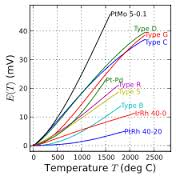
\includegraphics{Figures/thermocouple.jpg}
			\caption{Some calibration curves for different types of thermocouples. (PC: Wikipedia.org)}
		\end{center}
	\end{figure}
    
	Over the next few weeks, you will become very familiar with the sensors used in this course. We'll start by looking at the temperature sensor we'll be using for the semester. Unlike the thermocouple, this temperature sensor has a lot of processing circuitry built into it to make its calibration curve linear.
	
	\section*{How Analog to Digital Converters (ADCs) Work}
	In the previous lab, you probably figured out the form of the relationship between the raw voltage and value returned by analogRead(). However, it's unlikely you got this relationship exactly right, as that requires a slightly deeper understanding of how they work at the physical level. We wanted you to simply begin to think about how it worked before. Now, we'll cover this subject more deeply than both the prior lab and videos did.
	\\
	
	To begin, we have to consider the differences between the real world and the digital world. The digital world is essentially finite, whereas the real world is essentially continuous (we are going to ignore quantum mechanics). This means that when converting from the real world to the digital world, there will be some loss of information. This is an important fact to consider when evaluating a sensor or other tool.
	\\
	
	The ADC we're using in class is no exception - the maximum resolution, or how finely the instrument can be read, is controlled by the number of bits in the ADC. The more bits an ADC has, the higher the resolution. The equation below lets you calculate resolution. $V_{ref}$ is the maximum voltage of the ADC and bits is the number of bits in the ADC.
	$$ Resolution = \frac{V_{ref}}{2^{bits}} $$ 
	
    Now, to turn the raw value returned by analogRead() into a voltage, you need to simply multiply it by the resolution of the ADC. This is shown by the formula below.
    
    $$ Voltage = Value * Resolution $$
    
    Now, you may notice that this is a little odd. This would imply that a reading of 1023 from the ADC translates to a voltage of only 4.995V. However, last lab you saw that a value 5V gives you a reading of 1023! In addition, it would actually be impossible to ever calculate a voltage of 5V, as you would need a value of 1024 to get that.
    \\
      
    This is entirely due to how the information is quantized, or turned from the real world into the digital one. Basically, the graph of voltage versus analogRead() value looks like a series of steps. The final step in our plot starts at 4.995V and ends at 5V. The plot below shows an example for a 3-bit ADC. The x-axis shows you the fraction of $V_{ref}$ that produces the output of the ADC on the y-axis. This will be covered more in later lectures as well.
    
	\begin{figure}[h]
	\begin{center}
			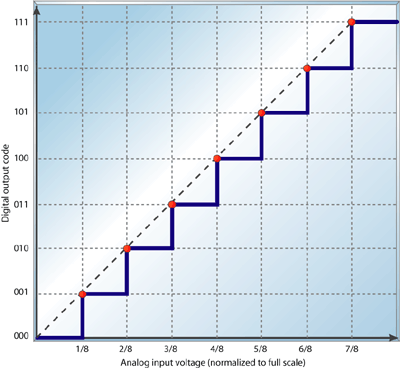
\includegraphics[scale = 0.6]{Figures/ADCplot.png}
			\caption{Photo Credit: embedded.com}
		\end{center}
	\end{figure}
    
    \newpage
	
	\section{Two-Point Calibration with the TMP36}
	\begin{enumerate}
	    
		
		\item Open the spec sheet provided for the temperature sensor. Identify the operating input current and output voltage ranges. Also take note of which pins must be connected to each circuit element. Connecting the TMP36 backwards will quickly smell like BBQ...
		This sensor is rather simple to interface with. When the temperature changes, the output voltage of the sensor changes as well. Below is a diagram demonstrating how the sensor should be connected to the Arduino.\\
		
	\begin{figure}[h]
		\begin{center}
			\begin{circuitikz} \draw
				(0, 2)	node[label={above:5V}]{}
				(0, 1)	to [short, -o]			(2, 1)
				(2, 1)	node[label={$V_{out}$}]{}
				(0, 0)	to [zD*, label={TMP36}]	(0, 2)
				(0, 0)	node[ground, label={[label distance = 0.8cm]below:GND}]{}
				;
			\end{circuitikz}
		\end{center}
		\caption{Temperature Sensor Circuit}
	\end{figure}

        \item Build the circuit and record the raw analogRead() value that the sensor outputs at the ambient temperature of the room. Do not convert to voltage. Additionally, record the room temperature reported by the thermostat in Celsius.
		
		\item Go outside and make another measurement. Allow a few minutes for the temperature value to settle - this will take a while, due to the thermal mass of the board.  You may want to leave your board outside for a bit of time. Record the outdoor temperature reported by a weather station in Celsius.
	
		\item Save the two coordinate pairs made up of the raw analogRead() values as well as the reported temperature in Celsius. You'll use these points to make a \textbf{two-point calibration} curve later in this lab. 
		
		\item Save your Arduino program, as you will be submitting it at the end of this lab.
	
\end{enumerate}
	
    \newpage
    \section*{The Thermistor}
    
	Next we'll use a temperature sensor with a simpler physical design that requires a bit more computational work to interpret. Like the thermocouple, this temperature sensor works due to internal changes in the material. As temperature increases, the electrons inside the device medium become more excited, allowing them to flow more easily. Thus, resistance decreases as temperature increases. This type of resistor is called a \textbf{Negative Temperature Coefficient (NTC) thermistor.} \\
    
    Unfortunately, unlike the characteristics of the TMP36, the calibration curve for the thermistors is pretty nonlinear, especially at low temperatures. Shown in Figure~\ref{fig:thermistor} is the approximate form of the temperature characteristic, as given in the spec for the part.\\
    
    \begin{figure}[h]
    	\begin{center}
        	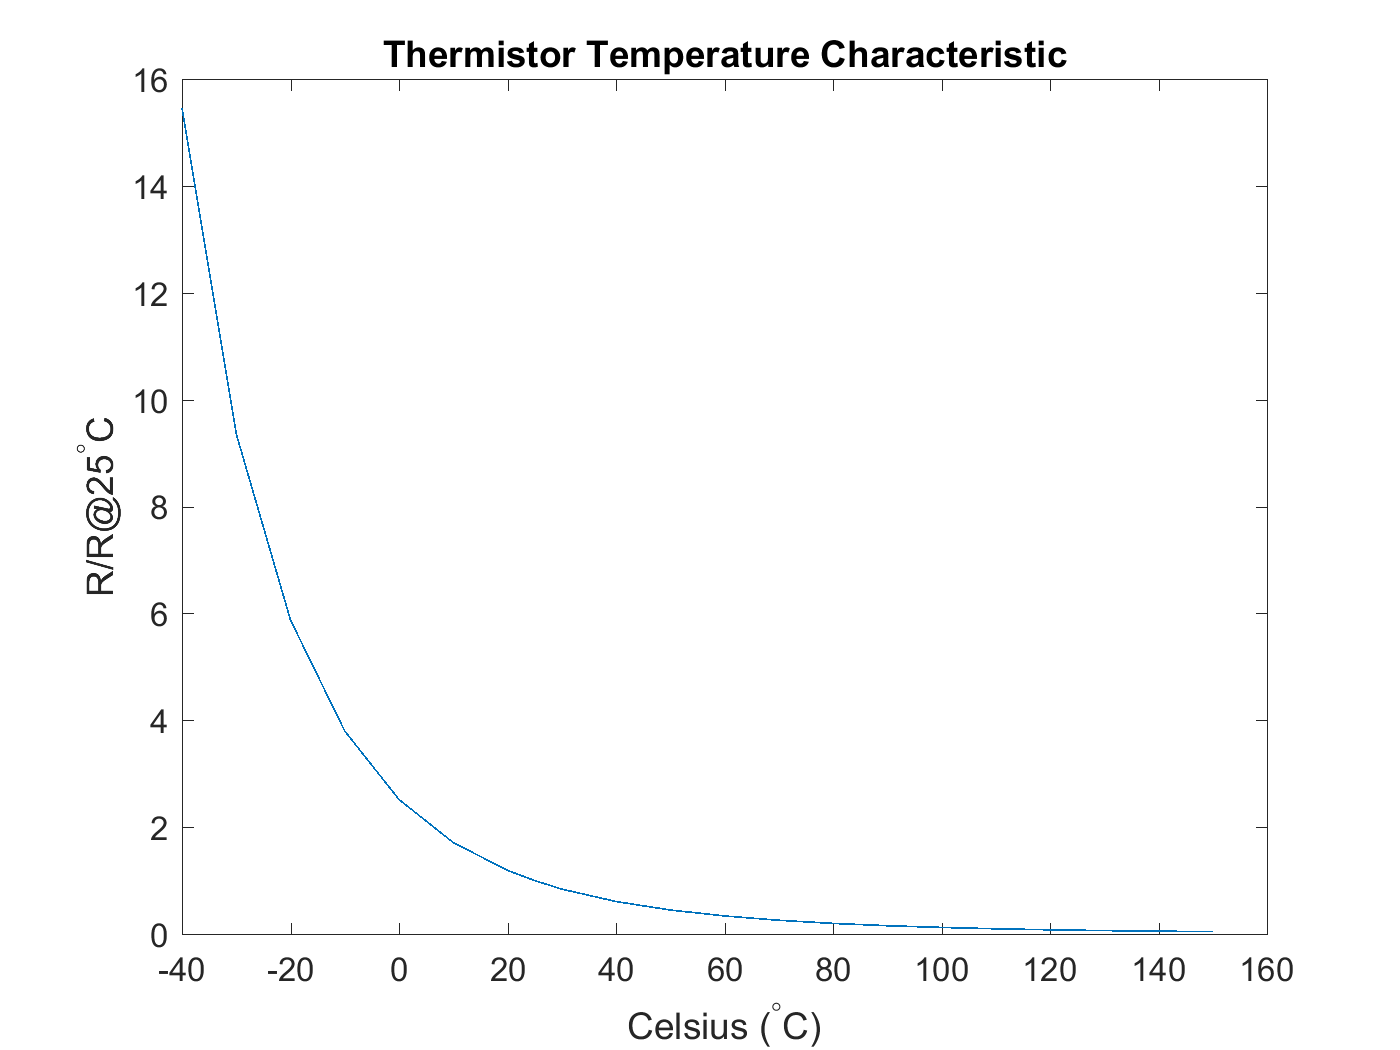
\includegraphics[scale=0.48]{Figures/therm_charac.png}
            \caption{An approximate thermistor characteristic.}
            \label{fig:thermistor}
         \end{center}
    \end{figure}
    
    The equation for the temperature as a function of the measured resistance of the device is given by:
    
    $$T(R) = \frac{B}{\ln({R/r_{\infty}})}, \textnormal{ where } r_{\infty} = R_0\hspace{1.5pt}e^{(-B/T_0)}$$
    
    $R_0$ is the resistance value at temperature $T_0$, which is usually taken to be room temperature (25$\degree$C/ 298 K). \textbf{When creating your curve, all temperature readings must be in degrees Kelvin for these equations to work properly.}\\
    
    We aren't done yet, though. Notice, the constant $B$ in the numerator and the argument of the exponential. This is called the `beta' of the thermistor, and is the most complex parameter of this equation. The beta can be estimated from two temperature/resistance measurements, $(R_1, T_1)$ and $(R_2, T_2)$ as
    
    $$B = \frac{\ln(\frac{R_1}{R_2})}{\frac{1}{T_1} - \frac{1}{T_2}}$$
    
    So we see that from only a few temperature measurements, we can approximate the behavior of the device over the entire temperature range. \textbf{Do the calibration in Kelvin.} \\
    
    This calibration curve is significantly more complicated than the linear two-point calibration curve that we used for the last lab.  It is probably a good idea in your MATLAB (or Python, or whatever code you use) to define the calibration constants at the top of your code (R0, R1, R2, T0, T1, T2), instead of hard-coding them into the main part of your code.  We should note that T0 and T1 can be the same measurement, which would make R0 and R1 the same too. You don't need 3 measurements for the curve, only 2!
    
    \newpage
    \subsection*{UART Communications}
    But we still have a rather inconvenient limitation on our system –- temperature readings can only be made manually, and aren't stored. Can we automate this reading, conversion, and storage process? Yes, because technology is awesome! \\
	
	Your launch payload is going to store results on an SD card, which will receive input directly from the Arduino. However, SD cards are designed such that they only can read communications formatted to a particular standard. This standard is called the \textbf{Serial Peripheral Interface (SPI)} and requires special libraries in order to be implemented with the Arduino. Instead, we'll use the communications hardware native to the Arduino, referred to as \textbf{Universal Asynchronous Receiver/Transmitter (UART)}, which is much simpler. In order to translate the data to SPI, we will include an intermediate temporary storage device, the OpenLog, meaning that you won't have to worry about SPI. The OpenLog will turn our UART communications into the SPI format that the SD card needs.
	
	We should take a few moments to discuss the UART communications protocol. First, we'll explain the basic necessities in any arbitrary communications protocol. \\
	
	You should be aware that a lot of information, such as simple integers and characters, can be encoded in sets of bits. These bits can either be 1 or 0 (binary), and combining them in different ways results in different values. As computers understand bits, a useful communications protocol must allow for data to be transmitted in sets of bits. These bits need to be communicated by some physical metric that both electronic devices can understand. We'll encode bits in voltage levels in this class. In the Arduino's case, a 5V signal represents a digital 1, and 0V signal represents a digital 0.\\
	
	Another important requirement is that each device needs to know when a new bit has been sent. That is, there needs to be some method to delineate between the bits within a message. This is actually more challenging of a problem than you might think. There are many ways to do this, and each has their own strengths and weaknesses.\\
	
	The final requirement we'll discuss today is the potential for two-way communications. Ideally, a communications protocol would allow for each device to send messages to the other when necessary. This, again, can be fairly complex to implement. \\
	
	Now we'll discuss how the UART communications protocol satisfies the above requirements. In UART, messages are sent in data frames of five to nine bits in size along with some additional overhead. The data frames are what contain the actual content of the message that we care about. In this class, we'll always send packets with eight data bits. \\
	
	Each message begins by drawing the voltage on a transmission line from high to low. After the start signal, the actual data of the message is sent inside of what is called the data frame. Each message ends with a stop bit where the line is pulled and kept high for the time it takes to send one bit (more on timing later). Each message also can have a parity bit, which can be used for error checking. We won't worry about parity bits in this class. Check out figure 1 below for a visual representation of a UART message. All messages sent in this class will have eight data frame bits, one stop bit, and one start bit. This means each message has ten bits, two of which are necessary overhead.

	\begin{figure}[h]
		\begin{center}
			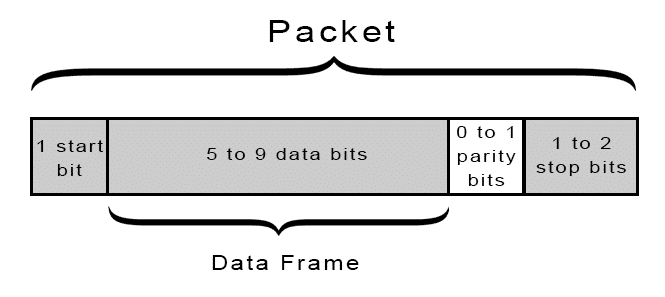
\includegraphics[scale=1]{Figures/UARTmessage.png}
			\caption{A typical UART message. Photo Credit: circuitbasics.com}
		\end{center}
	\end{figure}
	
	Now we need to discuss how bits are separated within a UART message. In UART, both devices that are communicating need to agree on a specific communications rate. That is, each device needs to know beforehand how much time there is between each bit. The individual devices use their own internal clocks to keep track of the time to make sure they understand each other properly. If the devices don't know beforehand what the data rate is, communications are essentially impossible. \\
	
	The data rate is also known as the baud rate, which is how many bits are sent per second. You should recognize this term from when you were printing to the Serial monitor in the prior labs. We'll use 9,600 baud in this lab. WiFi also has a baud rate.  Typical WiFi can have rates of 10Mbps (Mega-bits per second, so about 1000 times faster than the Arduino communicating with the computer).\\
	
	The final thing to discuss is how two-way communications are achieved. Each device that communicates over UART uses two pins, the RX and TX pins to accomplish this. TX stands for transmit, and RX stands for receive. Note that these are with respect to the particular device. {\bf The TX pin of one device needs to be connected to the RX device of the other for communications to work properly.} The digital signals are sent over these pins.
	
	\newpage
	\subsection*{The Level-Shifter}
	
	The OpenLog operates on a 3.3V input voltage and expects the digital inputs to have a maximum voltage of 3.3V on its communication lines. Our Arduino, however, outputs digital signals of either 0V or 5V. This higher voltage could potentially damage the OpenLog, and thus we can't communicate with it directly. We will use a logic Level-Shifter instead. This Level-Shifter will take the digital 5V logic of the Arduino and convert it into 3.3V logic (it can also do the reverse as well). \\
	
	The Level-Shifter is shown below. It is actually a generic device in that it can shift between two different arbitrary voltages.  For our application, these voltages are 5.0V and 3.3V. In order to do this, we have to provide the level-shifter these voltages, therefore, it requires references to (read: electrical connections to) the two voltages that you're trying to convert between -- in our case, 5V on the high voltage pin, and 3.3V on the low voltage pin. Since there are two references, there are two grounds, one on either side of this device, that both need to be connected to Arduino ground.
	
	\begin{figure}[h]
		\begin{center}
			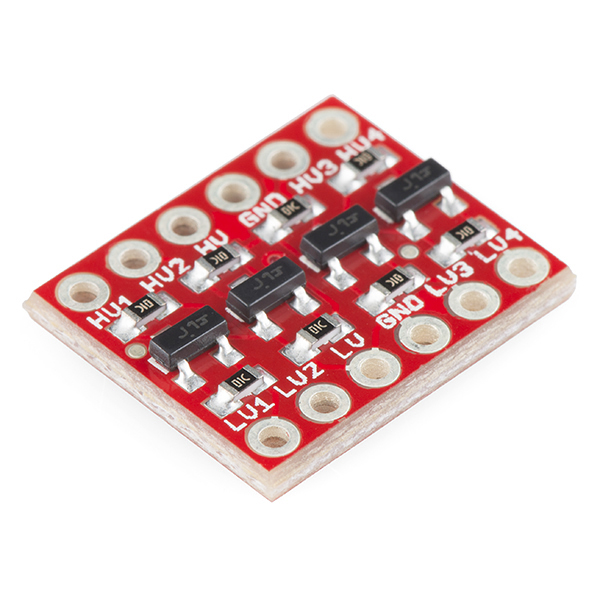
\includegraphics[scale=0.3]{Figures/level-shifter.jpg}
			\caption{The Level-Shifter component you will be using today.}
		\end{center}
	\end{figure}
	
	Apart from the voltage references, there are the high and low voltage channels. The Arduino outputs logic on a scale of 0-5V and the OpenLog should receive information on a scale from 0-3.3V. Keep in mind which side of the Level-Shifter is the low side and which is the high side when connecting components -- reversing them could be bad.
    
	\newpage
	
	\section{Adding the Thermistor and Writing Data}
	\begin{enumerate}
		\item Keep your TMP36 setup intact. Now build your thermistor sensor circuit. Recall that the thermistor acts like a resistor whose resistance varies with temperature. One way to measure the thermistor's resistance would be to use a voltage divider circuit. Use just the 1 k$\Omega$ resistor and the thermistor in this voltage divider.
		
		\item This time we'll be writing the data from our sensors to an SD card. Begin by identifying the pins of the OpenLog, and what they do. The BLK and the GRN pins can be safely ignored.
	
		\item Your Arduino Nano is designed with a built in receiving pin (RX) and a transmitting pin (TX). However, we won't be using them to connect to the OpenLog. Identify two arbitrary digital pins and connect them to the receiving and transmitting pins of the OpenLog via the Level Shifter. One will be a software assigned RX pin, and the other, a software assigned TX pin. We're going to be using a special library to designate digital pins on the Arduino as serial receive/transmit ports. Make sure you remember which is the TX and which is the RX pins! This is critical for your program to work correctly and mixing them up a very common mistake!
		
		\item Create a new Arduino program. At the top of your Arduino code, type: \\ \texttt{\#include $<$SoftwareSerial.h$>$}
		
		\item Declare a global variable using this library by \\ \texttt{SoftwareSerial variablename(RX, TX);} \\ where RX and TX are the receiving and transmitting pins you designate. You can now use \texttt{variablename} the same way you would use Serial.
		
		\item Be sure to initialize your serial port using the setup command: \\ \texttt{variablename.begin(9600);}
	
		\item Keep track of the elapsed time your Arduino has been running using the millis() function. Be sure you understand how to use it. Try printing just time data to the SD card to verify your setup works properly. Use: \\ \texttt{variablename.println(timevariable);}
		
		\item Send the voltage value read by the Arduino from the thermistor and TMP36 to the OpenLog. Recall our discussion on how to convert from analogRead() data to voltage. You simply multiply the resolution of the ADC by the value analogRead() returns. Write your result using: \\ \texttt{"variablename.println(result);"} \\
		
		Your script should be nicely formatted on the SD card as comma separated values. The first line of the script (in setup) can be labels for the columns. In the above case for instance, the data file might begin: \\
			\texttt{Voltage1,Voltage2,Time\\
			3.3,3.1,234\\
			3.4,3.3,248\\
			...}
		
		\item Run your code to gather the ambient room temperature measurement for both sensors. After that, ask one of the instructors to put your circuit inside of the dry ice chamber. We'll leave it in there for several minutes. Make sure your system is setup to constantly record the time and voltage values for both temperature sensors so we can eventually see how the system varies with time. Make sure to measure the temperature about once a second, but not significantly more than that.
	
		\item Save the data that you recorded for both sensors into a text file.
		
		\item Save your Arduino program, as you will be submitting it at the end of this lab.
	
	\end{enumerate}

    
	\section{Calibration and MATLAB Plotting}
	You will create a total of three plots in this section.
	\begin{enumerate}	
	    \item Plot 1: Make a two-point calibration curve for the TMP36, based on the two measurements you made indoors and outdoors. This curve should map directly from voltage to degrees Celsius. Keep in mind the discussion earlier in the lab about how ADCs work.
	    
	    \item On the same plot, make a calibration curve for the TMP36 using the data collected by the OpenLog in the dry ice chamber. 
	    
	    Make sure to include a title and appropriate axis labels. Plot these values over a range that makes sense. Consider the final project of the course in determining what range to plot over. Include a legend so we can tell which line is which.
		
		\item Plot 2: Now make a calibration curve for the thermistor using the data collected by the OpenLog in the dry ice chamber.
	
		\item Plot 3: Plot the temperature change as a function of time using the output in the SD card. Be sure to include correct time increments, axes-labels, and a legend. Do both the TMP36 and thermistor on the same plot. 
		
		It might be helpful to subtract out the minimum time value so that measurements start at $t = 0$.
		
		\item Also, note that your graphs are rather messy. There's a special filtering function \textbf{sgolayfilt()} in MATLAB that is useful for smoothing out curves by approximating sections of them with polynomials. It takes 3 parameters, a vector of y-axis values, the order of the approximation polynomial, and a 'frame length.' set the order to 2 and the frame length to 19. 
		
		Clean up your data by writing a for loop that repeatedly applies sgolayfilt() to your y-axis values until the amplitude of the oscillating values at room temperature is equal to or less than 5 mV.
	\end{enumerate}

	\section*{Post Lab Questions}
	For this lab, you and your partner may discuss the questions but must submit unique answers to the post lab questions. 
	
	\begin{enumerate}
	    \item Make a schematic that shows how the Arduino, TMP36, thermistor, LevelShifter, and OpenLog connect. Include any necessary resistors. For your reference, both components can be represented by boxes, with their pins labelled. For example, the TMP36 can be represented as shown below:
		
		\begin{figure}[h]
		\begin{center}
			\begin{circuitikz} [baseline=(current bounding box.center)]
				\ctikzset { label/align = straight }
				\draw
				(1, 2)		to[short, label={$V_{out}$}]	(2, 2)
				(-1, 1.35)	to[short, label={$V_{in}$}]	(-2, 1.35)
				(-1, 2.65)	to[short, label={GND}]	(-2, 2.65)
				(0, 2)	node[draw,minimum width=2cm,minimum height=2.4cm]{TMP36};
			\end{circuitikz}
			\caption{Temperature Sensor Block}
		\end{center}
		\end{figure}
	
		{\raggedright{}Alternatively, you could have all three pins on one side, or all pins on different sides, or some combination thereof. Your diagram should only include the two boxes for the components and lines connecting the pins appropriately.}
		
		Now on your diagram, indicate with arrows the flow of information between your Arduino and all of its peripherals (stuff that's attached). Be as specific as you can about where information is transmitted and received on each component.
	    
	    \item What  value  does  the  TMP36 spec  give  for  the  slope  and  intercept  of  it's  calibration  curve? Given this information, what would the voltage be at 25, 50 and 100 degrees Celsius?

		\item Using your two-point voltage/temperature calibration curve for the TMP36, calculate what the voltage would be at 25, 50, and 100 degrees Celsius. Repeat this calculation for the calibration curve using the dry ice chamber data. 
		
		Compare the voltage values calculated with your calibrations to the ones calculated using the spec sheet's calibration. How far off are the measurements from your calibrations?
		
		\item Resolution is defined as the fineness to which an instrument can be read.  Given that we need to read in the voltages output by each temperature sensor via our Arduino, what is the maximum level of resolution we could attain from a temperature measurement using each sensor?  Assume that each temperature sensor can output the exact voltage that represents a particular temperature to any number of decimal places and there is no external noise in our system.
		
		\item Why do you think that, despite all the fancy circuitry inside the temperature sensors, calibrations still need to be made?
		
		\textbf{For the remainder of the post lab questions, use the data collected in the dry ice chamber for both sensors.} 
		
		\item Now we'll do some analysis of what could happen if our temperature data is slightly off when doing thermistor calibration. In this question, we'll alter the single temperature point you used to calculate B and $r_{\infty}$ only. Plot a calibration curve where this temperature is 1 K above what we had originally, and keep all other values the same. Do this again for a temperature 2 K above, and once more for 5 K above. Plot all of these on the same graph and include the plot in your postlab response. How dramatically did the curve change using these new values for T? Why should you care about this?
		
		\item What is the time constant of each sensor? You can get a decent physical definition of time constant from Wikipedia. Calculate it, don't take it off the spec. Define what the time constant means with respect to our temperature sensors.
		
		\item Compare your calculated time constant values for each sensor to the spec sheet values. For the TMP36 sensor, look at the graph in figure 17 of the spec sheet to determine this. The thermistor time constant is described as the thermal cooling time constant in its data sheet.
		
		\item Our temperature sensors have a time constant, implying that it takes them time to adjust after being exposed to a new environment. What do you think would happen if we were to subject the temperature sensor to an environment where the temperature rapidly (say 100s of times per second) changed between -100$\degree$C and 100$\degree$C? Don't give a numerical answer, simply describe how well the system would respond to such a strange temperature environment. What would happen if our sensor had a time constant of 0?
		
		\item When using a sensor, what would be an advantage of having a very small time constant?
		
	\end{enumerate}
    
    \section*{Documentation for Postlab}
    On Canvas, turn in the following files. Your answers to the post lab questions must be your own work, but the Arduino scripts and MATLAB work may be the same as your partner's.
    \begin{enumerate}
        \item A PDF containing all answers to the post lab questions and all MATLAB plots created for this lab.
        \item The Arduino code (.ino) you used to create a two-point calibration with the TMP36.
    	\item The Arduino code (.ino) you used to record data from the dry ice chamber with the TMP36 and thermistor.
    	\item The text file (.txt) containing the data recorded in the dry ice chamber.
        \item The MATLAB code (.mat) used to create plots for this lab.
    \end{enumerate}
\end{document}
